\section{Incrementally maintain views in data analysis tasks}\label{sec: maintain_views}
%road map
In this section, some recent works on incrementally maintaining views in the data analysis environment are presented, in which the views can be machine learning model parameters \cite{deshpande2006mauvedb, gupta2015processing}, classification results by applying machine learning models \cite{koc2011incrementally} or the output of the general linear algebra programs \cite{nikolic2014linview}. Those works are introduced in the following three subsections respectively. \eat{The first one is to maintain materialized model parameters in database, which initially originates from  and follows by some other papers such as  while the other one is to maintain the classification results by the model, which is from .}

% develop a system (MauveDB vs Hazy) to store typical statistical model parameters as database view in RDBMS and update the views incrementally when raw data are modified.   

\subsection{Incrementally maintain model parameters}\label{sec: maintain_model_para}
%brief description to MauveDB
In this subsection, \cite{deshpande2006mauvedb} and parts of \cite{gupta2015processing} are presented, which regard the machine learning model parameters as database views and handle the changes over those models incrementally. In \cite{deshpande2006mauvedb}, the authors developed a system called MauveDB, which primarily deals with wireless sensor network applications, where data are collected through underlying sensors, trained with typical machine learning models such as regression-based model and interpolation-based model and used for estimating missing or future results. 
% The statistic models learned with those raw data are materialized as {\em model-based views}.
% , which are created with a high-level SQL-like language. 
The raw data from the underlying sensors are changing constantly, which requires efficient view maintenance strategies. 
Compared to \cite{deshpande2006mauvedb}, parts of \cite{gupta2015processing} also deals with the same problem but richer types of machine learning models, which, ultimately, goes towards the reuse of models in analytical workloads. In general, there are multiple ways to maintain the model parameters once the model is constructed, e.g. always computed from the scratch. Different model maintenance strategies introduced in \cite{deshpande2006mauvedb} and the details on incremental maintenance of model parameters for each machine learning algorithms are provided as follows.
% which highly depend on the types of statistical model.



\eat{\subsubsection{View definition}

MauveDB developed an declarative SQL-like language for users to define model-based view, which is exemplified in Figure \ref{fig:MauveDB_view_def}. Although different models cannot be manipulated in exactly the same way due to their different characteristics, the commonalities are still leveraged in this language. 

In Figure \ref{fig:MauveDB_view_def}, examples of regression-based view and Interpolation-based view definitions are presented in (i) and (ii) respectively. Same as way to create other database views, the view schemas, where the raw data comes from to construct the views (represented by \textit{SELECT}, \textit{FROM}) and what conditions the raw data should satisfy (represented by \textit{WHERE}) should be declared in the view definition statements. The model types (\textit{FIT} and \textit{INTERPOLATE} for regression and interpolation respectively) should be also specified along with partitions of raw data on each of which the models are trained (\textit{FOR EACH}) and other model-related information (such as base function for regression model, represented by \textit{BASE}). After executing statements shown in Figure \ref{fig:MauveDB_view_def}, {\em model-based views} are then created and stored in the RDBMS as relational tables.


\begin{figure}
    \centering
    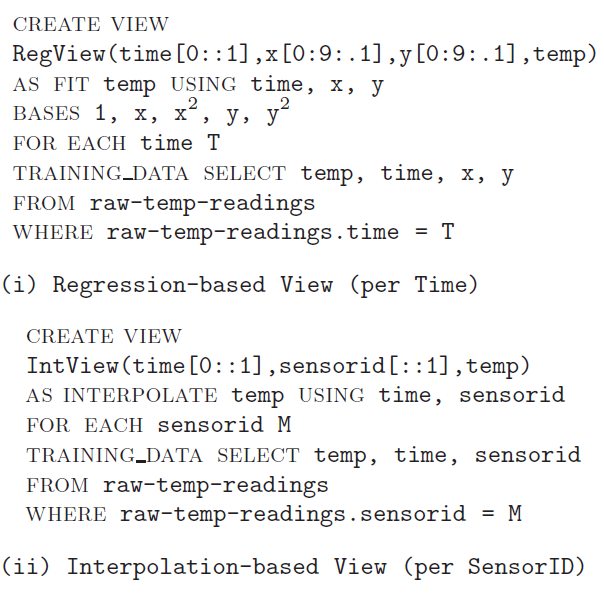
\includegraphics[width=8cm, height=8cm]{Figures/MauveDB_create_view.png}
    \caption{Define views in MauveDB}
    \label{fig:MauveDB_view_def}
\end{figure}
}
\subsubsection{View maintenance strategies}
%High-level descriptions of view maintenance strategies
When new data are available, the updates should be reflected on the model-based views. Four different strategies are developed in MauveDB for this purpose and their trade-offs are discussed with extensive experiments. The details of the four view maintenance strategies are introduced as below.

\textit{Strategy 1: Materialize the views}
A naive way is simply to construct the models and materialize the model parameters as views in the database, which can avoid unnecessary query execution time when users want to retrieve the ``exact'' model information. However, such views may incur high space overhead and pose a challenge in refreshing the model as new data comes.

\textit{Strategy 2: Always use the base data }
This strategy goes to another extreme without materialization at all in the database, which can obviously make query processing very expensive since recomputating the view content is necessary every time when queries are evaluated. 

\textit{Strategy 3: Partial materialization}
Somewhere in-between is to partially materialize the view content, which simply caches parts of the views that have been computed by certain queries. When the views are about to be refreshed, the corresponding cached contents in memory will be invalidated.

\textit{Strategy 4: Materialize an intermediate representation}
Some intermediate representations are materialized in this strategy by leveraging some nice properties of the machine learning models, which have been proven to be an efficient solution by experiments and are presented below for each model respectively.

The specific choice of strategies in practice depends on various factors, such as the query workload, data statistics and types of models. The trade-off between the four strategies are experimentally explored with extensive experiments in \cite{deshpande2006mauvedb}, which shows that the strategy 4 performs best in most scenarios.

\subsubsection{View maintenance for each model}\label{sec: view_maintenance_model}
\paragraph{view maintenance for regression model} \cite{deshpande2006mauvedb} and \cite{gupta2015processing} apply strategy 4 over the regression model in the same way. Recall that the optimal coefficients can be solved with Equation \ref{eq: regression_solve}. The intermediate representation for it can be simply the materialization of matrix $H^TH$ and $H^T\bar{y}$, which can be beneficial in various aspects. First, the dimensions of the two matrices only rely on the total number of features, which thus won't lead to large space overhead. Besides, efficient updates to the two matrices are achievable since they are computed with linear operators, i.e. matrix multiplications and additions. A newly generated data point $(\bar{x}',\bar{y}')$ can trigger the update of $H^TH$ and $H^TY$ as follows:
\begin{equation}
    (H^TH)^{new}_{i,j} = (H^TH)^{old}_{i,j} + h_i(\bar{x}')*h_j(\bar{x}')
\end{equation}
\begin{equation}
    (H^TY)^{new}_i = (H^TY)^{old}_i + h_i(\bar{x}')*\bar{y}'^T
\end{equation}

Where $(H^TY)^{x}_i$ ($x \in \{old, new\}$) represents the $i_{th}$ entry in the vector $(H^TY)^{x}_i$. Once $H^TH$ and $H^TY$ are updated, the coefficient $W$ is computed with Equation \ref{eq: regression_solve_final}, 
% \begin{equation}
%     \bar{w}^*=(H^TH)^{-1}H^T\bar{y}
% \end{equation}
which can be computed with time complexity $Q(k^3)$ where $k$ is the total number of basis functions. As mentioned before, in the simplest case when $H=X$, i.e. $H_i(*)$s are all identity functions and the number of basis functions is the same as the number of features, then $k$ also represents the number of features.

\paragraph{View maintenance for interpolation model} \cite{deshpande2006mauvedb} also processes interpolation model by applying strategy 4, in which the data in the interpolation-based view $\textbf{V}$ will be of the form $(\textbf{t}, \textbf{v})$ where $\textbf{t}$ and $\textbf{v}$ represent predictor variable and response variable respectively. Unlike regression mode where the intermediate representations are the intermediate computation results, the intermediate representations of interpolation model are some auxiliary data structure for searching the values of variable $\textbf{t}$. When new data point $(t', v')$ is inserted into the $\textbf{V}$, then the data structure should be updated to reflect the effect of the insertion such that when predicting the value for $\textbf{v}$ given $\textbf{t}$ value $t''$, the values of $t_{i}$ and $t_{i+1}$ used in Equation \ref{eq: interpolation} for the prediction can be efficiently retrieved with the updated data structure from $\textbf{V}$.
% In order to efficiently estimate the value of $\textbf{v}$ given the value of $\textbf{t}$, $t'$, which is missing from the view instance but queried by users, the closest $\textbf{t}$ values $t_{-}$ and $t_{+}$ (along with the corresponding $\textbf{v}$ values $v_{-}$ and $v_{+}$) to $t'$ are retrieved with the auxillary data structure such that $t'$ lies in the interval $(t_{-}, t_{+})$ without any other $\textbf{t}$ value from $\textbf{V}$ inside the interval. So the estimated $\textbf{v}$ value for $t'$ can be computed using Equation \ref{eq: interpolation}.


\paragraph{View maintenance for Naive Bayes model}
As mentioned before, \cite{gupta2015processing} deals with richer types of machine learning models such as Naive Bayes model and logistic regression model, which still follows the ideas of strategy 4 to maintain the model-based views. In terms of Naive Bayes model, based on Equation \ref{eq: nb_exp} and Equation \ref{eq: nb_guassian}, the membership probability depends on the values of $n_c$, $\mu_{jc}$ and $\sigma_{jc}^2$, in which $\mu_{jc}$ and $\sigma_{jc}^2$ require the sum and square of sum of the feature values within the class $c$, i.e. $\Sigma_{i=1}^n(x_{ij}I(y_i=c))^2$ and $\Sigma_{i=1}^nx_{ij}I(y_i=c)$ (denoted as $SS_{jc}$ and $S_{jc}$ respectively) from Equation \ref{eq: nb_mean} and \ref{eq: nb_var}, which are thus materialized. When a new data point $\bar{x}, y$ comes where $\bar{x}^T = [x_1, x_2, \dots, x_d]$, $n_c$, $S_{jc}$ and $SS_{jc}$ is updated as:

\begin{equation}
    \begin{split}
        n_c' &= n_c + I(y=c)\\
        S_{jc}' &= S_{jc} + x_jI(y=c)\\
        SS_{jc}'&= SS_{jc} + x_j^2I(y=c)\\ &= SS_{jc} + (x_jI(y=c))^2
    \end{split}
\end{equation}

\paragraph{View maintenance for logistic regression model}
Unlike the machine learning models discussed above, there is no closed-form solution for logistic regression model, which requires gradient descent algorithm with non-linear operator (i.e. logistic function) involved to derive the model parameter $\bar{w}$ in Equation \ref{eq: logistic_regression_prob}. 

As the first step toward incrementally maintaining the logistic regression model, a variant of statistical gradient descent, i.e. Mixture Weight Methods \cite{mcdonald2009efficient} is used, which is sketched in Algorithm \ref{alg: mixture weight method}. Intuitively, this algorithm splits the entire dataset into $p$ partitions in the beginning and the size of each partition is $l$. For $i_{th}$ partition, the gradient descent algorithm is applied to derive the model parameter (denoted by $\bar{w}_i$). In the end, the model parameters computed from every partition are averaged as the final output. Then given the training data points $\{\bar{x}_i, y_i\}_{i=1}^n$ on which Algorithm \ref{alg: mixture weight method} is applied, the model parameter derived from each partition is materialized, which forms a parameter set $P = \{\bar{w}_1, \bar{w}_2, \dots, \bar{w}_p\}$. 

To incrementally update the model parameter, the new data points due to the updates are also split into partitions of size $l$ and the model parameter for each partition is derived by applying SGD as Algorithm \ref{alg: mixture weight method} proceeds, which is also added into $P$. In the end, the updated model parameter $\bar{w}^{new}$ is computed by averaging the parameters from the updated $P$. According to \cite{mcdonald2009efficient}, the gap between $\bar{w}^{new}$ and the model parameter computed over the updated training data set from the scratch is bounded.


\begin{algorithm}[h!] 
\footnotesize
%  \SetKwInOut{Input}{Input}
%  \SetKwInOut{Output}{Output}
%  \Input{a set of valid view mappings $\mathcal{M}$ for query tuple $t \in Q(D)$, query $Q$}

%  \Output{a set of covering sets $C$}
 Partition $\{\bar{x}_i, y_i\}$ into $p$ partitions, $\{S_1, S_2,\dots, S_p\}$, each of which is of size $l$.
 
 \For{all $i \in \{1,2,\dots, p\}$}
 {
    $\bar{w}_i \leftarrow 0$
    
    \For{$t \leftarrow 1$ to T}
    {
        \tcp{ $F_{S_i}(\bar{w}) = \frac{1}{|S_i|}\Sigma_{(\bar{x}_i, y_i) \in S_i}L(\bar{w};\bar{x}_i, y_i) + \lambda R(\bar{w})$, which is adapted from Equation \ref{eq: logistic_objective_function}}
        $\triangledown F_{S_i}(\bar{w}) \leftarrow GRADIENT(F_{S_i}(\bar{w}))$
    
        $\bar{w}_i \leftarrow \bar{w}_i + \lambda(\triangledown F_{S_i}(\bar{w}))$
    }
 }
 
 Aggregate all $\bar{w}_{\mu} = \Sigma_{k=1}^p\mu_k\bar{w}_k$    
 
 \caption{Mixture weight method}
 \label{alg: mixture weight method}
 \end{algorithm}




\subsection{Incrementally maintain classification result}\label{sec: maintain_classification}
Hazy \cite{koc2011incrementally} is a system, aiming at incrementally maintaining classification results such that the performance of the read and update operations over the classification results are optimized, which mainly supports typical linear machine learning algorithms, including support vector machines, ridge regression and logistic regressions.

\subsubsection{Views in Hazy}


\eat{\begin{figure}
    \centering
    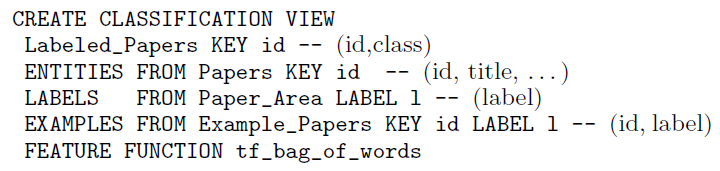
\includegraphics[width=10cm, height=2.5cm]{Figures/Hazy_view.png}
    \caption{Define views in Hazy}
    \label{fig:Hazy_view_def}
\end{figure}}

%intro to view definition
In Hazy, the goal is to classify a set of entities (samples) with some classifier. Each entity has the form $(id, \bar{f})$, where the $id$ is the entity id while $\bar{f}$ is the feature values for this entity. \eat{users can declare views in the way shown in Figure \ref{fig:Hazy_view_def}, in which a {\em classification view} is defined over some entity table (i.e. $Papers$ in Figure \ref{fig:Hazy_view_def}, with Primary key $id$) to identify their type (i.e. $Paper\_area$) with a model trained using some training examples (i.e. $Examples\_papers$) that are derived from original entity table by applying some feature function (i.e. $tf\_bag\_of\_words$ function). So in the end, }The view content is composed of the classification results for each entity, in which each tuple has the form $(id, class)$ where $class$ is the label determined by the machine learning model for the entity with identifier $id$. There are two strategies to store the view content, i.e. {\em eager strategy} and {\em lazy strategy}. The major difference between the two strategies is that the former one stores the materialized views in the database while the latter one only keeps views virtual.

%operations in Hazy and the bottleneck for eager and lazy approach
Hazy focus on three typical {\em queries} issued by the users: 1) {\em Single entity} read, i.e. retrieve the label of a single entity; 2) {\em All members} read, i.e. retrieve the labels for all the entities; 3) {\em Update}, i.e. update the classification results in the view content once the model is updated due to some incoming new training examples. Intuitively, the {\em update} should become the bottleneck for eager approach since the materialized views should be refreshed whenever updates happen while the {\em All members} read should be the major overhead for lazy approach since the content of the virtual views should be computed whenever read queries are issued, which are the major concerns for the authors of Hazy. In terms of {\em update} queries, the authors assume that the time to retrain the model is negligible (roughly on the order of 100$\mu$s on their datasets) and the major overhead for view maintenance is to relabel the entities in the materialized views for eager approach. 

\subsubsection{Overview of view maintenance in Hazy (eager approach)}
%overview of view maintenance problem
In what follows, the details on how to maintain materialized classification views in Hazy are provided, which targets at more efficient {\em update} queries for eager approach rather than recomputing the content of views from the scratch when updates happen. Lazy approach is free from this issue since updates won't influence the virtual views in the database. 

%introduce notation for table H
Every time when updating the views is defined as an {\em epoch}. Suppose support vector machine is used thereafter (other classifiers are also applicable and introduced later) for binary classifications (extensions for multiple classifications are introduced later), at epoch $i$, the model parameters will be $(\bar{w^{(i)}}, b^{(i)})$. Given an entity with feature vector $\bar{f}$, its label is determined by the sign of the residual $eps = \bar{w^{(i)}}\cdot\bar{f}-b^{(i)}$. If $eps > 0$ ($eps < 0$ respectively), then this entity is labeled as $+$ ($-$ respectively).

Recall the assumption that the time to retrain the model is not significant, the model is firstly retrained at each epoch. Given the updated model parameters, a scratch table $\textbf{H}$ is maintained inside Hazy, which stores tuples of the form $(id, \bar{f}, eps)$ where $id$, $\bar{f}$ and $eps$ represents the entity id, feature vector and residual (computed by $eps = \bar{w^{(i)}}*\bar{f}-b^{(i)}$). Then the classification view $\textbf{V}$ can be obtained from $\textbf{H}$, in which each view tuple has the form $(id, c, eps)$ ($c$ is the label for entity with identifier $id$ and is calculated as $c=sign(eps)$). 
%For a tuple $t \in \textbf{H}$ ($\in \textbf{V}$ resp.), we use $t.attr$ denote the value of attribute $attr$ at tuple $t$ where $attr$ is an attribute of $\textbf{H}$ ($\textbf{V}$ respectively). For example, $t.\bar{f}$ and $t.id$ represent the feature vector and the entity at tuple $t$ in $\textbf{H}$.

%introduce two steps
\paragraph{Incremental step VS reorganization step} At epoch $i$, the scratch table $\textbf{H}$ is represented as $\textbf{H}^{(s)}$ which indicates that $\textbf{H}$ is constructed at epoch $s$ ($s < i$) and keeps the same after epoch $s$ until epoch $i$, view $\textbf{V}^{(i+1)}$ can be either {\em incrementally} constructed from $\textbf{V}^{(i)}$ by updating small portion of view tuples in $\textbf{V}^{(i)}$ without changing $\textbf{H}^{(s)}$ or computed by referencing latest $\textbf{H}$ which is {\em reorganized} at epoch $i$ (i.e. $\textbf{H}^{(s)}$ becomes $\textbf{H}^{(i)}$). Intuitively, the {\em incremental} step is relatively cheaper since it only touches parts of the view content and does not modify $\textbf{H}$. However, compared to the model constructed at epoch $s$, which is the latest {\em reorganization step}, more and more tuples in $\textbf{V}$ need to be updated since current model may be far away from the model at epoch $s$ as the time goes by. So the {\em reorganization step} is needed at some point to reduce the overhead to update the labels in $\textbf{V}$ in the following {\em incremental steps}.

%cost of the two options
\paragraph{Cost measure and skiing strategy} Due to the existence of two alternative choices at each epoch, i.e. {\em incremental step} and {\em reorganization step}, we should determine whether {\em incremental step} or {\em reorganization step} is taken at each epoch such that the overall overhead is minimized. A sequence of the choice of {\em reorganization step} or {\em incremental step} at each epoch is defined as a {\em strategy}. In order to determine the optimal strategy, Hazy quantifies the cost for the {\em incremental step} and {\em reorganization step} and formalizes it as the classic {\em ski rental problem} \cite{karlin1994competitive}. In this problem, the cost of the {\em incremental step} is defined as the time to update $\textbf{V}^{(i)}$ to $\textbf{V}^{(i+1)}$, which should be proportional to the view tuples relabeled at epoch $i$ (denoted as $c^{(i)}$) while the {\em reorganization step} has a fixed cost $S$. Suppose the {\em reorganization step} is taken at epoch $s$, then the accumulated cost at epoch $i$ by applying {\em incremental step} since epoch $s$ is $a^{(i)} = \sum_{j=s+1}^ic^{(j)}$. The strategy ({\em skiing strategy}) is as follows: If the accumulated cost $a^{(i)}$ is too large, say, greater than $\alpha S$ ($\alpha$ is a constant), then refresh table $H$ (the accumulated cost $a^{(i)}$ is reset to 0 after that). This strategy is proven to be 2-approximation asymptotically compared to the optimal strategy.


\subsubsection{Details of incremental step}\label{Sec: incremental step}
%overview
The core idea of {\em incremental step} is to do small changes over the classification view to reflect the model updates, the details of which are presented as below. It starts by introducing how to determine which part of view tuples to be changed at each epoch with two thresholds, which follows by the detailed derivation rules of the two thresholds.

\paragraph{Thresholds in incremental step}
%intro to lower water and higher water
For incremental step, it is assumed that the appearance of the new training examples do not result in great changes to the model, which means that it is safe to simply update small portion of the view content to achieve performance gains at each epoch. Intuitively, the labels of the entities that are far away from (close to resp.) the decision boundary should be less likely (more likely resp.) to be flipped when the updates happen. Its effect is presented in Figure \ref{fig:Hazy_view_update}, in which the model targets at classifying database papers. The small variation over the model, i.e. $\delta_w$ over $w$, has no influence on the labels of the samples far away from the decision boundary such as entity $P_4$.

\begin{figure}
    \centering
    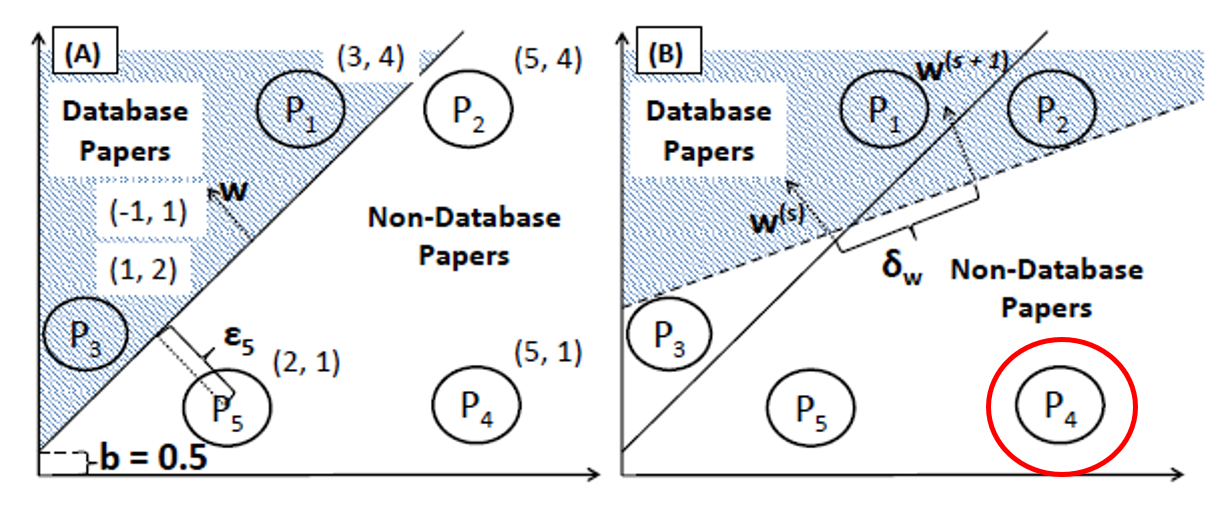
\includegraphics[height = 0.3\textwidth, width=0.6\textwidth]{Figures/Hazy_view_update.png}
    \caption{The effect of small updates on the model over the views}
    \label{fig:Hazy_view_update}
\end{figure}


To determine which samples should be relabeled or not at each epoch, Hazy introduces two thresholds, lower water and higher water (denoted by $lw$ and $hw$ respectively, which are negative and positive respectively). At each epoch $i$, by referencing the residual value $eps$ for each entity in the scratch table $\textbf{H}^{(s)}$ computed at epoch $s$ ($s<i$), if $eps$ is greater than $hw$ (less than $lw$), then the labels of the corresponding entities are guaranteed to be $+$ ($-$ respectively) and thus remain unchanged. The process is exemplified in Figure \ref{fig:Hazy_threshold}, in which the entities to be reclassified are highlighted.


\begin{figure}
    \centering
    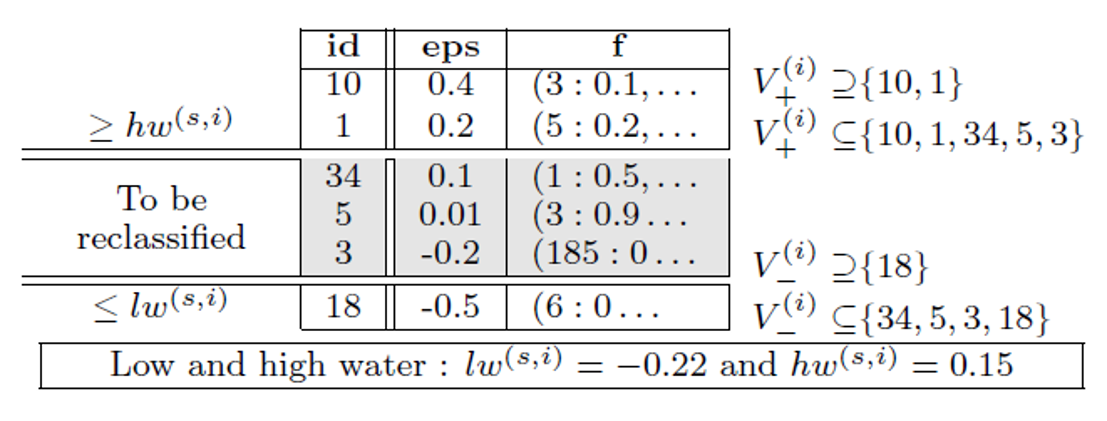
\includegraphics[height = 0.3\textwidth, width=0.6\textwidth]{Figures/Hazy_threshold.png}
    \caption{Determining the entities to be relabeled in the view in incremental step}
    \label{fig:Hazy_threshold}
\end{figure}

%how to compute lower water and higher water
\paragraph{How to determine the thresholds}
Intuitively, the two thresholds $hw$ and $lw$ should be adjusted at each epoch $i$ since the differences between model at epoch $i$ and model at epoch $s$ (when $\textbf{H}$ is recomputed) may be varied for different $i$. So $hw$ and $lw$ are associated with superscript $^{(s,i)}$ to indicate that they are related to the models at epoch $s$ and $i$, i.e. $hw^{(s,i)}$ and $lw^{(s,i)}$ respectively, which are computed as follows:

\begin{equation}
    lw^{(s,i)} = min_{l=s,\dots, i}\epsilon_{low}^{(s,l)},
    hw^{(s,i)} = max_{l=s,\dots, i}\epsilon_{high}^{(s,l)}
\end{equation}

where $\epsilon_{low}^{(s,l)}$ and $\epsilon_{high}^{(s,l)}$ are computed as (recall that $t.\bar{f}$ represents the feature vector of $t$):
\begin{equation}\label{eq: epsilon}
    \epsilon_{low}^{(s,l)} = -max_{t \in \textbf{H}}||t.f||_q||\bar{w^{(s)}}-\bar{w^{(l)}}||_p+b^{(l)}-b^{(s)}, \epsilon_{high}^{(s,l)} = max_{t \in \textbf{H}}||t.f||_q||\bar{w^{(s)}}-\bar{w^{(l)}}||_p+b^{(l)}-b^{(s)}
\end{equation}
where the norm $q$ and $p$ satisfy $p^{-1} + q^{-1} = 1$. Recall that $\bar{w^{(s)}}$, $b^{(s)}$ and $\bar{w^{(i)}}$, $b^{(i)}$ represents the model parameters at epoch $s$ and $i$ respectively.


There is a nice property by applying Holder's inequality \cite{rudin1976principles} to $\epsilon_{low}^{(s,j)}$ and $\epsilon_{low}^{(s,j)}$, i.e. at epoch $j$, for a tuple $t \in \textbf{H}^{(s)}$, if $t.eps \geq \epsilon_{high}^{(s,j)}$ ($t.eps \leq \epsilon_{low}^{(s,j)}$), then $t.id$ should be in the class $+$ ($-$). The proof is sketched as follows:

% Define $\delta \bar{w} = \bar{w}^{(j)}-\bar{w}^{(s)}$. 
\begin{proof}
To prove that $t.id$ is in class $+$ at epoch $l$, we need to prove that $t.f\cdot \bar{w}^{(l)} - b^{(l)} > 0$. According to Equation \ref{eq: epsilon},
$\epsilon_{high}^{(s,l)} = max_{t \in \textbf{H}}||t.f||_q||\bar{w^{(s)}}-\bar{w^{(l)}}||_p+b^{(l)}-b^{(s)} \geq ||t.f||_q||\bar{w^{(s)}}-\bar{w^{(l)}}||_p+b^{(l)}-b^{(s)}$. By applying Holder's inequality, we have $||t.f||_q||\bar{w^{(s)}}-\bar{w^{(l)}}||_p \geq ||t.f||||\bar{w^{(s)}}-\bar{w^{(l)}}|| \geq ||t.f \cdot(\bar{w^{(s)}}-\bar{w^{(l)}})||$. $\epsilon_{high}^{(s,l)} = max_{t \in \textbf{H}}||t.f||_q||\bar{w^{(s)}}-\bar{w^{(l)}}||_p+b^{(l)}-b^{(s)} \geq ||t.f||_q||\bar{w^{(s)}}-\bar{w^{(l)}}||_p+b^{(l)}-b^{(s)} \geq ||t.f \cdot (\bar{w^{(s)}}-\bar{w^{(l)}})|| + b^{(l)}-b^{(s)} \geq t.f \cdot (\bar{w^{(s)}}-\bar{w^{(l)}}) + b^{(l)}-b^{(s)}$. Note that $t.eps = t.f \cdot \bar{w}^{(s)} - b^{(s)}$ If $t.eps \geq \epsilon_{high}^{(s,l)}$, then $t.eps \geq t.f \cdot (\bar{w^{(s)}}-\bar{w^{(l)}}) + b^{(l)}-b^{(s)} = t.eps - t.f \cdot \bar{w}^{(l)} + b^{(l)}$, which means that $t.f\cdot \bar{w}^{(l)} - b^{(l)} > 0$.
\end{proof}

\subsubsection{Details of reorganization step}
The {\em reorganization step} for the scratch table $\textbf{H}$ includes recomputing the residual $\epsilon$ for each entity in $\textbf{H}$, reconstructing necessary indexes to quickly search the entity in $\textbf{H}$ and sorting the entire table by the residual $eps$.\eat{, which happens when the current model is far away from the model computed in the last reorganization step. A greedy strategy is proposed earlier to determine whether {\em reorganization step} or {\em incremental step} is chosen at each epoch.  Formally speaking, when the cost of {\em reorganization step} (fixed as $S$, which is the time to perform the {\em reorganization step}) is less than the accumulated cost $a_{i}$, {\em reorganization step} is executed.}

\subsubsection{Analysis of the greedy strategy}
Two assumptions about the cost measure are made for {\em skiing strategy}: 1) the cost of incremental step, $c^{(s, i)}$ only depends on the current epoch $i$ and the most recent epoch $s$ for reorganization step since $c^{(s, i)}$ is a function of the number of tuples within the interval $[lw^{(s,i)}, hw^{(s,i)}]$; 2) Reorganization more recently won't increase the cost $c^{s,i}$, which means that $c^{(s, i)} < c^{(s',i)}$ for $s > s'$. The assumptions above can guarantee 2-approximation compared to theoretical optimal strategy. The analysis is sketched as follows.


%notations
Recall that the total overhead for reorganization step is $S$, in which the time to scan $\textbf{H}$ is $\sigma S$. Given $N$ epochs in total, reorganization step is executed $M$ times, which happens at epoch $\mu_1, \mu_2,\dots, \mu_M$ ($0 \leq \mu_1 < \mu_2 < \dots < \mu_M \leq N$), The integer sequence $\bar{\mu} = \mu_1, \mu_2,\dots, \mu_M$is defined as a {\em schedule} under a certain strategy. At any epoch $i$, we define $\floor{i}_{\bar{\mu}} = max\{\mu \in \bar{\mu} | \mu < i\}$, which intuitively returns the most recent epoch before epoch $i$ when {\em reorganization step} is executed. Denote the set of costs for every epoch by $\bar{c} = \{c^{(s,i)}\}$, the total cost of a {\em schedule} will be:
\begin{equation}\label{eq: cost}
    Cost(\bar{\mu}, S, \bar{c}) = \sum_{i=1,2,\dots,N}c^{(\floor{i}_{\bar{\mu}}, i)} + MS
\end{equation}

Equation \ref{eq: cost} indicates that the total cost not only depends on how to schedule the reorganization step, but also depends on the cost at each epoch, i.e., $\bar{c}$ and $S$. This is because at each epoch, the value of $c^{(\floor{i}_{\bar{\mu}}, i)}$ is known to us only after the model is updated and thus $\epsilon^{(s,l)}_{low}$ and $\epsilon^{(s,l)}_{high}$ in Equation \ref{eq: epsilon} can be derived. (recall that $c^{(s,i)}$ is related to the interval $[lw^{(s,i)}, hw^{(s,i)}]$ and $lw^{(s,i)}$, $hw^{(s,i)}$ are derived from $\epsilon^{(s,l)}_{low}$ and $\epsilon^{(s,l)}_{high}$), which can influence the accumulated cost $a^{(i)}$ and thus influence the decision (recall that the decision at epoch $i$ depends on whether $a^{(i)}$ is greater than $\alpha S$). So given a strategy $\Phi$, the schedule $\bar{\mu}$ should be a function of $\bar{c}$, i.e. $\bar{\mu} = \Phi(\bar{c})$.

In order to prove that the skiing strategy is a 2-approximation strategy, the {\em competitive ratio} (denoted by $\rho$) is defined as below, which is a ratio between the cost of a strategy $\Phi$ and and the optimal cost:
\begin{equation}
    \rho(\Phi) = sup_{\bar{c}}\frac{Cost(\bar{\mu}, S, \bar{c})}{Cost(\bar{o}, S, \bar{c})}
\end{equation}


where $\bar{o}$ represents the optimal schedule. It is proven that $\rho(skiing) = (1+\alpha + \sigma)$ where $\alpha$ is the positive root of $x^2 + \sigma x - 1$ and for any other deterministic strategy, $\rho(\Phi) \geq (1+\alpha + \sigma)$. Specifically, when the number of entities goes to infinity, the time to scan $\textbf{H}$ table, i.e. $\sigma S$ should be approaching 0 (recall that $S$ is the reorganization time, which includes the time to sort $\textbf{H}$. The sorting time is more expensive than scanning time). In this case, $\alpha \rightarrow 1$ and thus $\rho(skiing) \rightarrow 2$.

% The proof of $\rho(skiing) = (1+\alpha + \sigma)$ is sketched as follows:
% 
% \begin{proof}
% 1) first we prove that $\rho(skiing) = (1+\alpha + \sigma)$. 

% Suppose the {\em reorganization step} happens at epoch $t_1, t_2, \dots, t_M$. Consider any interval $[t_m, t_{m+2})$, in which the cost in the interval $(t_m, t_{m+1})$ and $(t_{m+1}, t_{m+2})$ is $C_1$ and $C_2$ respectively. So the total cost in this interval would be $C_1 + C_2 + S$. Since the reorganization step happens at epoch $t_{m+1}$ and $t_{m+2}$ respectively, it means that $C_i \geq \alpha S$ ($i=1,2$) according to the skiing strategy. Besides, at epoch $t_{m+1}$, 


% \end{proof}

\subsubsection{Overview of read queries in Hazy (lazy approach)}
%overview
In this section, how Hazy improves the performance on read queries, i.e. {\em single entity} read and {\em all members} read is presented. Recall that in eager approach, the classification views are materialized. So read queries are not a bottleneck here since the labels of either single entity or all the entities can be retrieved from the view instance directly. On contrast, only the virtual views are used in lazy approach, which may slow down the read queries since the view content should be generated whenever read queries are issued. As a result, the authors focus on improving the performance of read queries (especially {\em all members} queries) for lazy approach.

Suppose a user wants to retrieve all the entities of the positive class, which is a typical {\em all members} query, in the naive solution, at a certain epoch $i$, all the entities need to be scanned to be labeled with the current model. However, in Hazy, not all the entities are needed to answer this query. Instead, by referencing the scratch table $\textbf{H}^{(s)}$ (reorganized at epoch $s$, $s < i$), only the tuples $t \in \textbf{H}$ satisfying $t.eps > lw^{(s,i)}$ are needed (recall that entities with residual $t.eps < lw^{(s,i)}$ are guaranteed to be in the negative class). 

Same as view maintenance problem introduced in the previous few sections, for eager approach, there also exists a trade-off on whether the scratch table $\textbf{H}$ should be reorganized. For the read queries under the lazy approach, the greedy strategy is applied to determine when to do reorganization but with different cost measure to quantify the overhead of {\em incremental step}. Suppose it takes $S'$ seconds to read the entire entities, the number of real positive entities is $N_{+}$ and the number of entities above the low water $lw^{(s,i)}$ is $N_{R}$, then the cost of {\em all members} queries will be $c^{(i)} = \frac{N_{R}-N_{+}}{N_{R}}S'$ and the accumulated cost is calculated as in Section \ref{Sec: incremental step}. Then the rest of the skiing strategy here is identical to the one used for eager approach.


\subsubsection{Other optimizations in Hazy}
Hazy also provides two types of system variants to achieve the performance enhancement. The first one is to maintain the classification views and the scratch table $\textbf{H}$ in memory (refered as Hazy-MM), which can be safely discarded when reorganizations happen since the model parameters will be recomputed at each epoch. The other one is to hybrid the main-memory structure and the on-disk structure to reduce the memory consumption. The performance trade-offs between the original system design and the two variants are explored experimentally.

\subsubsection{Extends to other machine learning models}
In the previous sections, it is assumed that the default machine learning algorithm is support vector machine and the problems Hazy is dealing with belong to binary classification problem. But Hazy is also flexible to handle other machine learning models (with kernel methods) and multi-class classification.

\paragraph{Other machine learning model}
Other linear classification models are also supported by Hazy, which includes ridge regression and logistic regression. Actually, typical linear classification model can be formalized as {\em convex optimization problem} to derive the best parameter $\bar{w}$, which has same form as Equation \ref{eq: logistic_objective_function} and is usually solved with gradient descent methods. Then the label of an entity with feature values $\bar{x}$ is determined as:

\begin{equation}
    l(\bar{x}) = h(\bar{w}\cdot\bar{x})
\end{equation}
% \begin{equation}\label{eq: opt_expr}
%     min_{\bar{w}}P(\bar{w}) + \Sigma_{(\bar{x},y) \in \textbf{T}}L(\bar{w}\cdot\bar{x}, y)
% \end{equation}

% where $\bar{x}$ is the feature vector, $P$ is the {\em regularization term} and $L$ is the {\em loss function}. Typical solution to optimize the objective function shown in Equation \ref{eq: opt_expr} is to apply gradient descent methods to derive $\bar{w}$ iteratively until it converges to $\bar{w}*$, which is then used to classify a certain sample with feature values $\bar{x}$ as follows:

where $h$ is simply sign function for binary classification problem.

Since the objective function of other linear classification models share the same form as support vector machine, it is pretty straightforward to migrate the solutions to those classification models.

\paragraph{Kernel methods}
Kernel methods extend linear classification models with kernel function $K: \mathbb{R}^d \times \mathbb{R}^d \rightarrow \mathbb{R}$, which is a positive semi-definite function. Given a kernel function, the corresponding classification function would be:
\begin{equation}\label{eq: kernel classification}
    l(\bar{x})=h(\Sigma_{i=1,2,\dots,N}c_i\cdot K(\bar{s_i}, \bar{x}))
\end{equation}
where $\bar{s}_i$ is the {\em support vector} and $c_i$ is the weight value for the $i_{th}$ kernel function. In this case, the weight vector $\bar{w}$ is: $\bar{w} = [c_1, c_2,\dots, c_N]$, which can still fit the eager approach and lazy approach proposed before.

%linearized kernels
Some further improvements can be applied to a special type of kernel functions called shift-invariant kernels, which satisfy $K(x, y) = K(x-y)$ where $K$ is a kernel function and regarded as a simple function. Shift-invariant kernels includes many common kernels, such as the Gaussian and the Laplacian kernel. By applying {\em random non-linear feature vectors} \cite{rahimi2008random}, $K(x, y) \approx z(x)^Tz(y)$ where $z$ is a random map: $\mathbb{S}^d \rightarrow R^D$ (suppose $x, y \in \mathbb{S}^d$), which can thus simplify Equation \ref{eq: kernel classification} as below:
\begin{equation}
    l(\bar{x})=h(\Sigma_{i=1,2,\dots,N}c_i\cots K(\bar{s_i}, \bar{x})) = h(\Sigma_{i=1,2,\dots,N}c_i\cots z(\bar{s_i})^T z(\bar{x}))=h(\bar{v}^T z(\bar{x}))
\end{equation}

where $v=\sum_{i=1,\dots,N}c_i z(\bar{s_i})$. This technique can substantially reduce the dimension.

\paragraph{Multi-class classification}
Hazy builds a decision-tree-like structure to turn a multi-classification problem to binary classification problem.

\subsubsection{Experimental results}
The authors also conducted experiments on three different datasets, i.e. Forest, DBlife and Citeseer to compare the time performance between the skiing strategy (Hazy) and Naive strategy under both on-disk and in memory architecture, which are presented in Table \ref{tab:hazy_exp}. In those experiments, the average time per update in Eager approach and the average time per {\em All members} read query in Lazy approach are recorded.

As Table \ref{tab:hazy_exp} shows, in most cases, Hazy achieves at least one order-of-magnitude speed-up relative to Naive implementation even in on-disk architecture. But there is still one exception on update queries over Citeseer datasets, in which Hazy fails to outperform Citeseer. The reason behind that is that Citeseer dataset has larger feature space and thus the model fails to converge by the end of each epoch, which forces Hazy to conduct more unnecessary reorganization steps and thus pay more cost on sorting operation in those steps. But in-memory architecture incurs much less overhead in sorting and thus Hazy is more efficient than Naive implementation.


\begin{table}[h]
    \centering
    \begin{tabular}{|c|c|c|c|c|c|c|c|}\hline
        && \multicolumn{3}{|c|}{Eager {\em Update} (updates/s)}&\multicolumn{3}{|c|}{Lazy {\em All members} (scan/s)}  \\\hhline{~~------}
        % &&Re-evaluation & Incremental\\ \hline
        &&Forest&DBLife & Citeseer & Forest & DBLife & Citeseer\\\hline
    \multirow{2}{*}{On disk}&Naive&0.4 & 2.1 & 0.2 & 1.2 & 12.2 & 0.5\\\hhline{~-------}
    &Hazy&2.0 & 6.8 & 0.2 & 3.5 & 46.9 & 2.0\\\hline
    % \multicolumn{2}{|c|}{Hybrid}&2.0 & 6.6 & 0.2 & 8.0 & 48.8 & 2.1\\\hline
    \multirow{2}{*}{In memory}&Naive&5.3 & 33.1 & 1.8 & 10.4 & 65.7 & 2.4\\\hhline{~-------}
    &Hazy&49.7 & 160.5 & 7.2 & 410.1 & 2.8k & 105.7\\\hline
    % \multirow{3}{*}{Space}&Linear & $n^2$ & $n^2k$\\\hhline{~---}
    % &Exponential & $n^2$ & $n^2log k$\\\hhline{~---}
    % &Skip-s & $n^2$ & $n^2(logs+\frac{k}{s})$\\\hline
    \end{tabular}
    \caption{Experiemental results in Hazy}
    \label{tab:hazy_exp}
\end{table}


% \subsection{Discussion}
